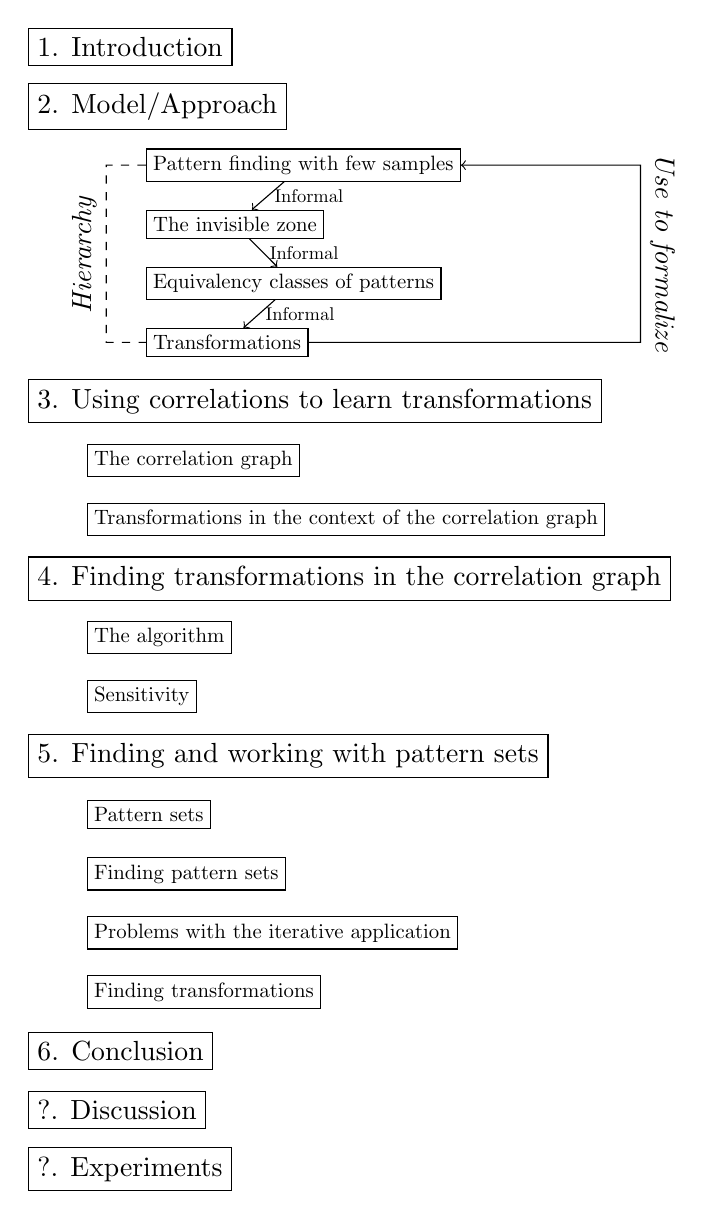
\begin{tikzpicture}[scale=0.75]
    \tikzset{box/.style={draw, align=left, anchor=west}}
    \tikzset{innerbox/.style={draw, align=left, anchor=west, scale=0.75}}
    
    \node[box] (Intro) at (0,0) {1. Introduction};
    \node[box] (Model) at (0,-1) {2. Model/Approach};
        \node[innerbox] (Pattern) at (2,-2) {Pattern finding with few samples};
        \node[innerbox] (Invisible) at (2,-3) {The invisible zone};
        \node[innerbox] (Classes) at (2,-4) {Equivalency classes of patterns};
        \node[innerbox] (Transformation) at (2,-5) {Transformations};
        \draw[dashed] (Pattern) to[out=180, in=0] (1.33,-2) --node[rotate=90, above] {\textit{Hierarchy}}++(0,-3) to[out=0,in=180] (Transformation);
        \foreach \i/\j in {Pattern/Invisible,Invisible/Classes,Classes/Transformation}{
            \draw[->] (\i)--node[right, scale=0.666, draw=none] {Informal} (\j);
        }
        \draw[->] (Transformation) --++(7,0)--node[rotate=-90, above] {\textit{Use to formalize}}++(0,3)to[out=180,in=0] (Pattern);
        
    \node[box] at (0,-6) {3. Using correlations to learn transformations};
        \node[innerbox] (CorrelationGraph) at (1,-7) {The correlation graph};
        \node[innerbox] (TrafosInCG) at (1,-8) {Transformations in the context of the correlation graph};
        
    \node[box] at (0,-9) {4. Finding transformations in the correlation graph};
        \node[innerbox] at (1,-10) {The algorithm};
        \node[innerbox] at (1,-11) {Sensitivity};
        
    \node[box] at (0,-12) {5. Finding and working with pattern sets};
        \node[innerbox] (PatternSets) at (1,-13) {Pattern sets};
        \node[innerbox] at (1,-14) {Finding pattern sets};
        \node[innerbox] at (1,-15) {Problems with the iterative application};
        \node[innerbox] at (1,-16) {Finding transformations};
    \node[box] at (0,-17) {6. Conclusion};
    \node[box] at (0,-18) {?. Discussion};
    \node[box] at (0,-19) {?. Experiments};
\end{tikzpicture}